\documentclass[border=10pt]{standalone}
\usepackage{pgfplots}
\pgfplotsset{compat=1.17}
\begin{document}
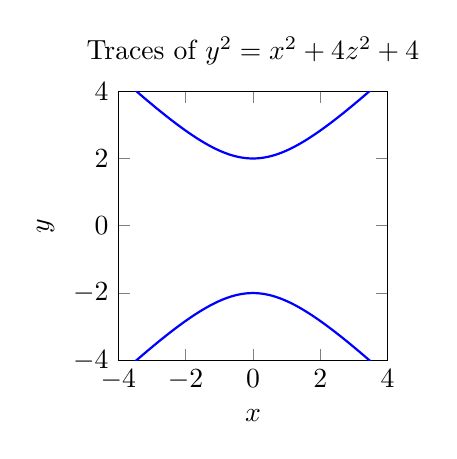
\begin{tikzpicture}
\begin{axis}[
    title={Traces of $y^2=x^2+4z^2+4$},
    xlabel=$x$, ylabel=$y$,
    xmin=-4, xmax=4, ymin=-4, ymax=4,
    axis equal,
    width=5cm, height=5cm,
    samples=100
]
\addplot[blue, thick, domain=-4:4] {2*sqrt(1+x^2/4)};
\addplot[blue, thick, domain=-4:4] {-2*sqrt(1+x^2/4)};
\end{axis}
\end{tikzpicture}
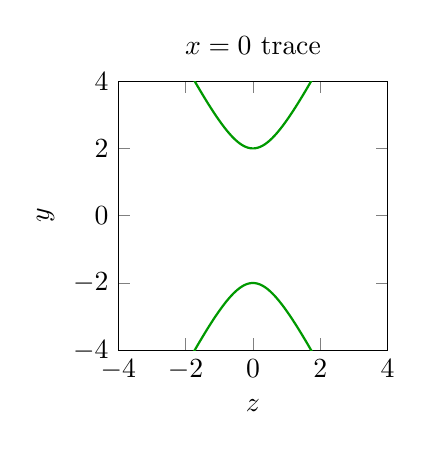
\begin{tikzpicture}
\begin{axis}[
    title={$x=0$ trace},
    xlabel=$z$, ylabel=$y$,
    xmin=-3, xmax=3, ymin=-4, ymax=4,
    axis equal,
    width=5cm, height=5cm,
    samples=100
]
\addplot[green!60!black, thick, domain=-3:3] {2*sqrt(1+x^2)};
\addplot[green!60!black, thick, domain=-3:3] {-2*sqrt(1+x^2)};
\end{axis}
\end{tikzpicture}
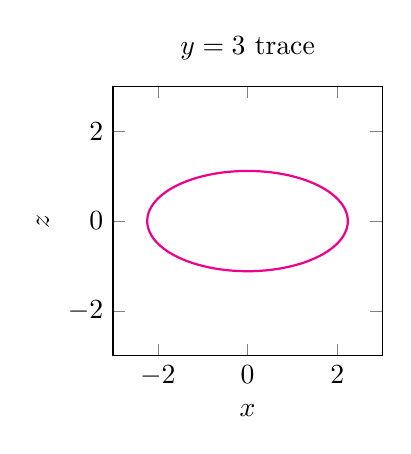
\begin{tikzpicture}
\begin{axis}[
    title={$y=3$ trace},
    xlabel=$x$, ylabel=$z$,
    xmin=-3, xmax=3, ymin=-2, ymax=2,
    axis equal,
    width=5cm, height=5cm,
    samples=100
]
\addplot[magenta, thick, domain=0:360, variable=\theta] ({2*sqrt(5/4)*cos(\theta)},{sqrt(5/4)*sin(\theta)});
\end{axis}
\end{tikzpicture}
\end{document}
